\clearpage
\chapter{Diagramme}
\section{UML-Diagramme}
\subsection{Idee/Erstes UML-Diagramm}
Miri: Das Erste UML-Diagramm entstand nach dem ersten Brainstorming in der Analysephase. Alle Teammitglieder disskutierten über das mögliche Spielkonzept. Dabei wurden die ersten Ideen gesammelt und aufgrund der Ideen wurde das erste UML-Diagramm entwickelt. \\
Nach weiteren Besprechungen und zu Beginn Fachkonzept, aufgrund des UML-Diagramms umzusetzen, sind verschiedene Fehler aufgetreten, die wir so nicht implementieren konnten. 
Beispiele der Fehler waren, dass die einzelnen Uhren in dem Unternehmen erzeugt werden müssen, sonst hat der Spieler keinen Zugriff darauf oder dass ein Spielbrett zur Verwaltung des ganzen Spielablauf gefehlt haben.

\begin{figure} [h]
	\centering
	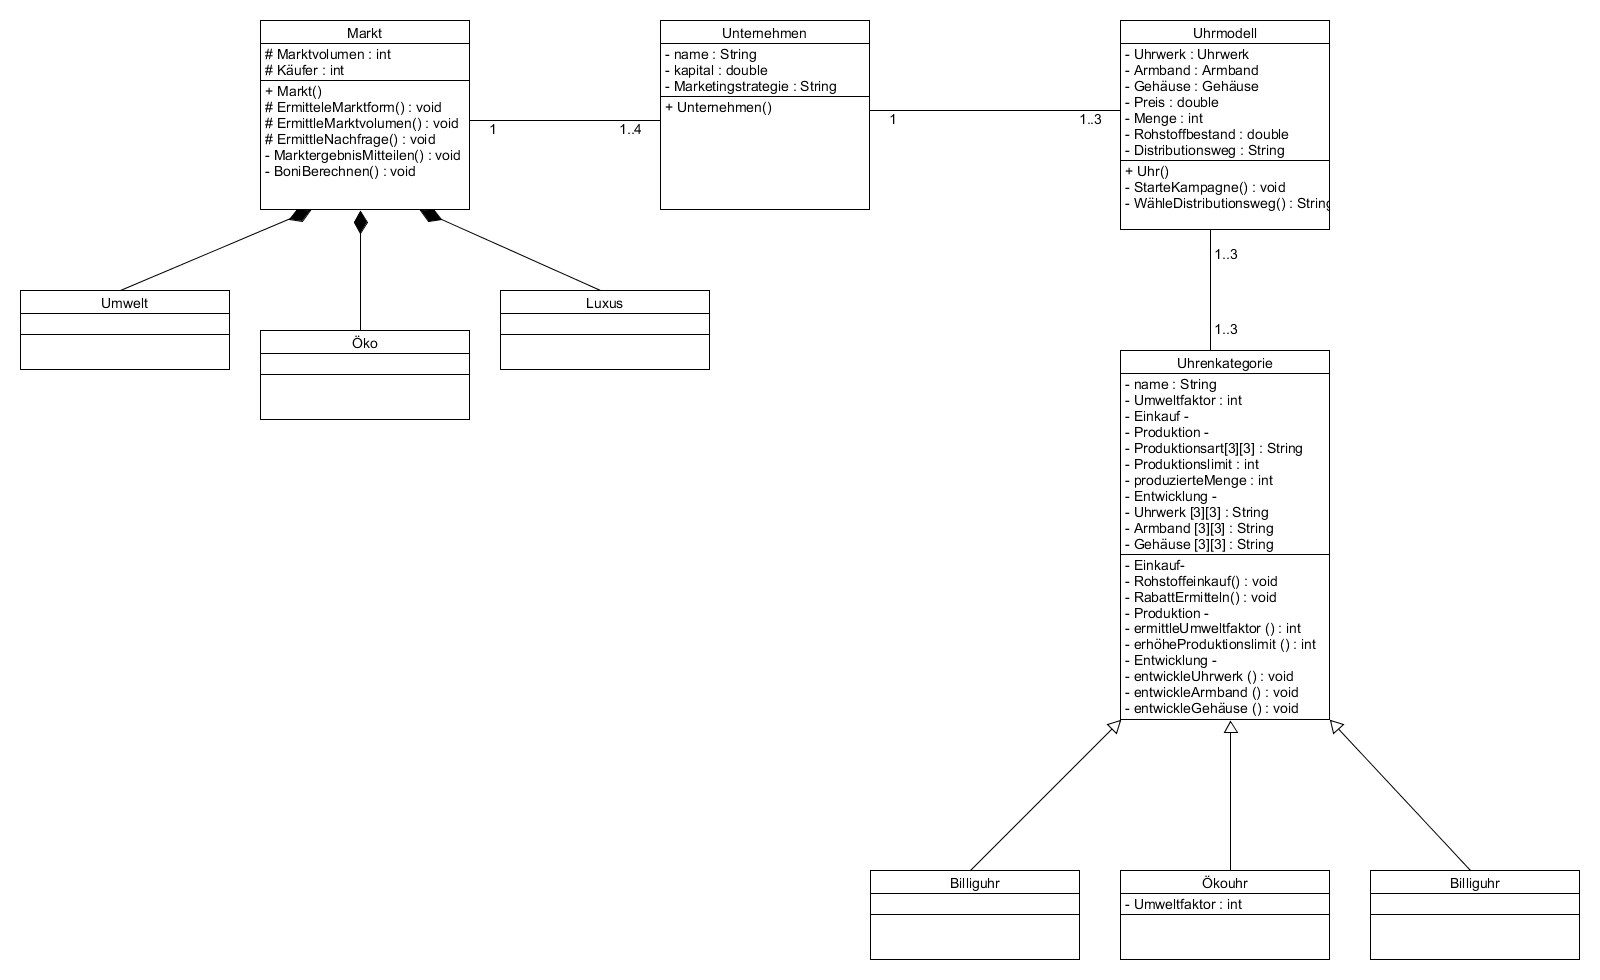
\includegraphics[scale=0.25, angle=90]{img/ErsterEntwurfUML.png} 
	\label{key}
	\caption{text}
\end{figure}
\clearpage
\subsection{Finales UML/Unternehmenssimulation}
Miri: Das Finale UML-Diagramm der Unternehmenssimmulation entstand bei der Erstellung des Fachkonzeptes. Während der Entwicklung des Diagrammes wurden mehrere Meetings gehalten, das UML-Diagramm verbessert und die Entwürfe ins Fachkonzept umgesetzt. Die anstehenden Fehler wurden wiederum im nächsten Meeting besprochen und das Diagramm angepasst. Am Ende der Entwicklungsphase war das Finale UML-Diagramm fertig.
\begin{figure} [!h]
	\centering
	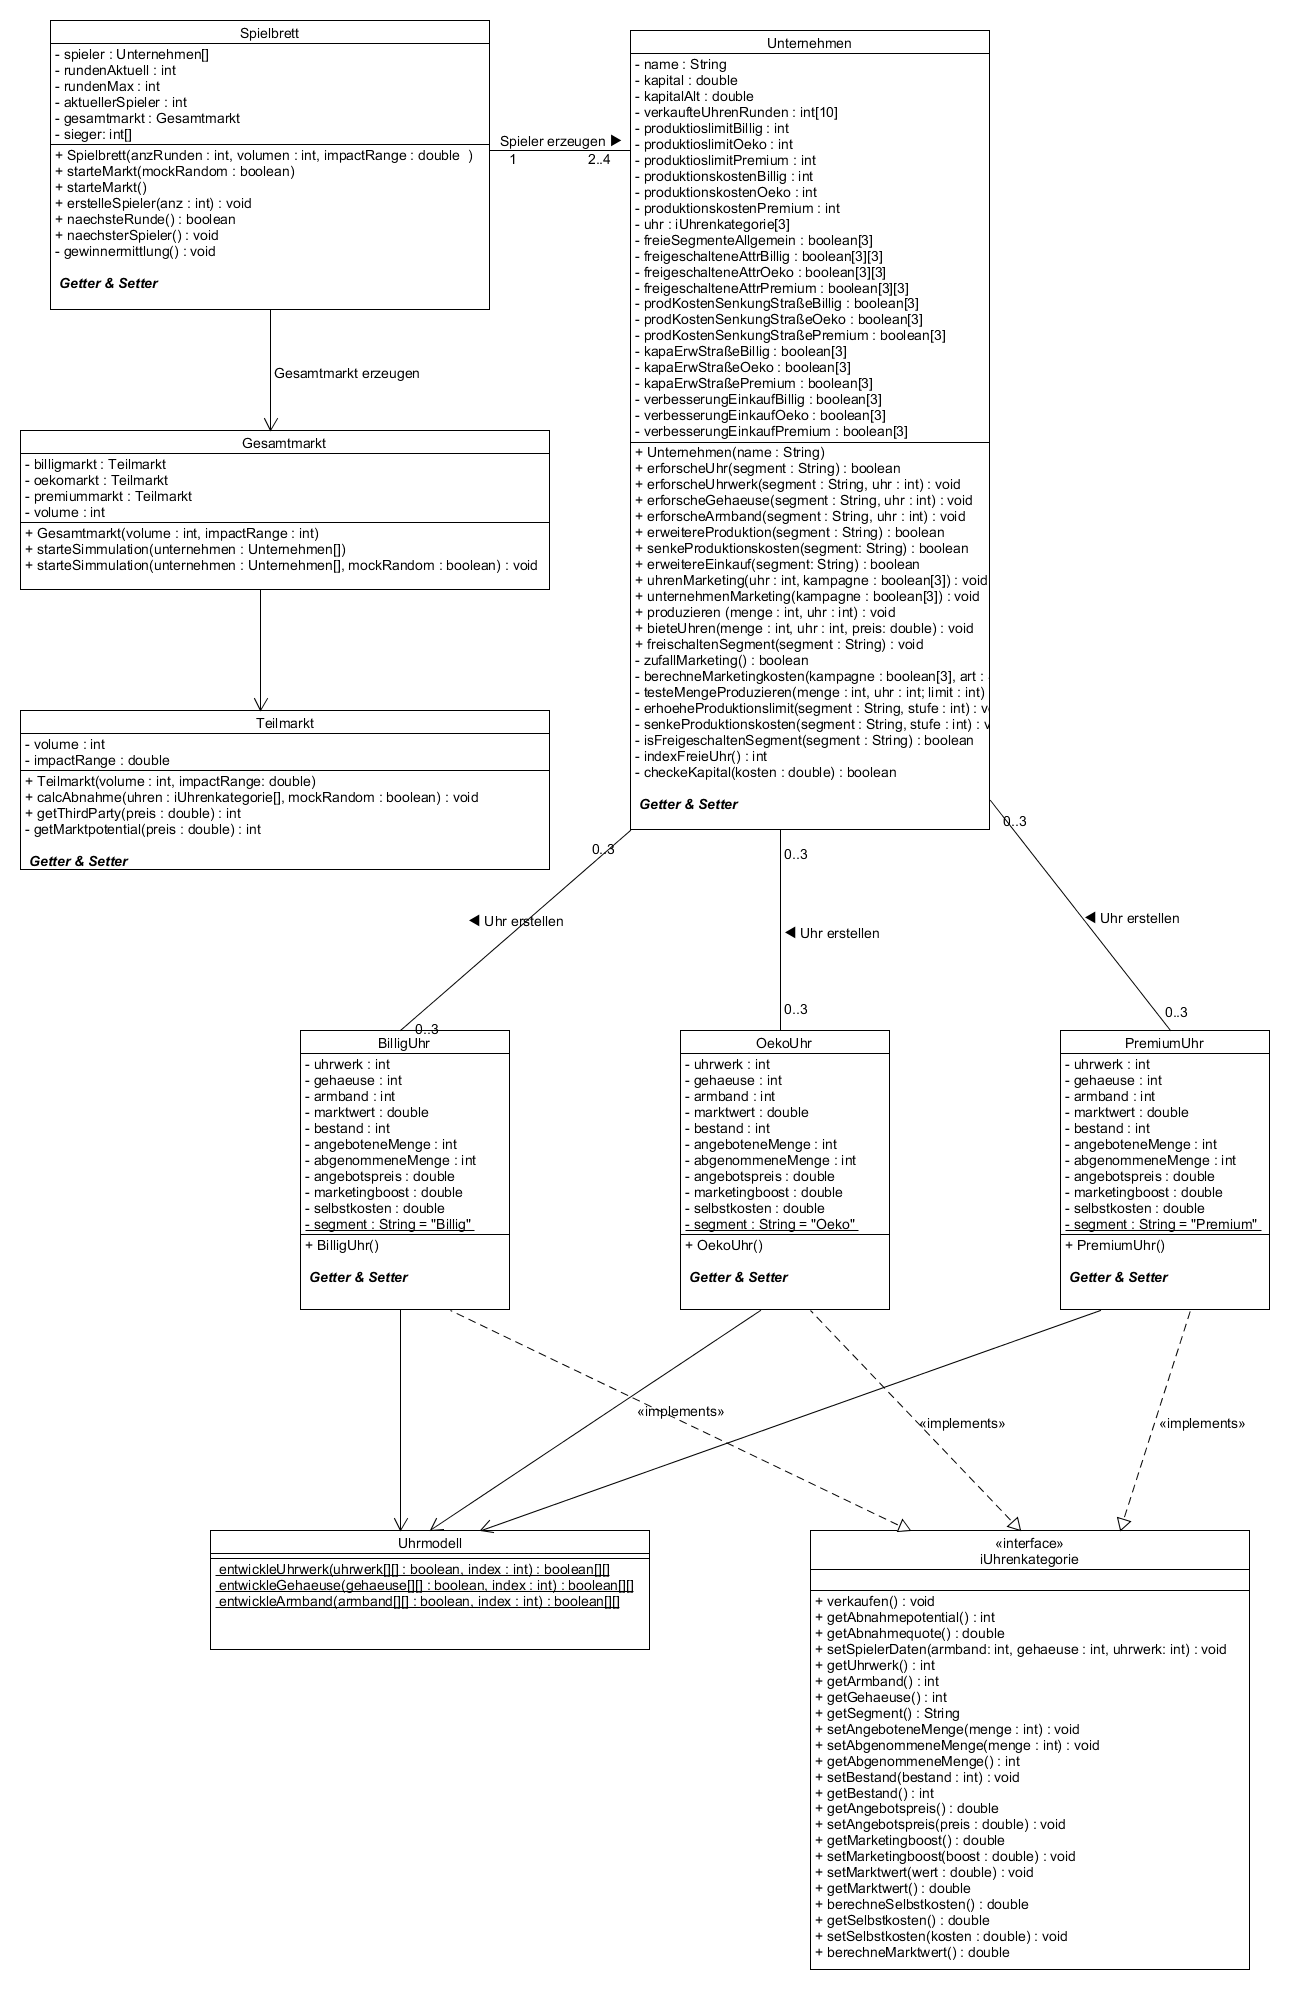
\includegraphics[scale=0.36]{img/Unternehmenssimmulation_final.png} 
	\label{UML-Final}
	\caption{text}
\end{figure}
\clearpage
\section{Ablauf-UML}
\subsection{Spielablauf}
\begin{figure} [!h]
	\centering
	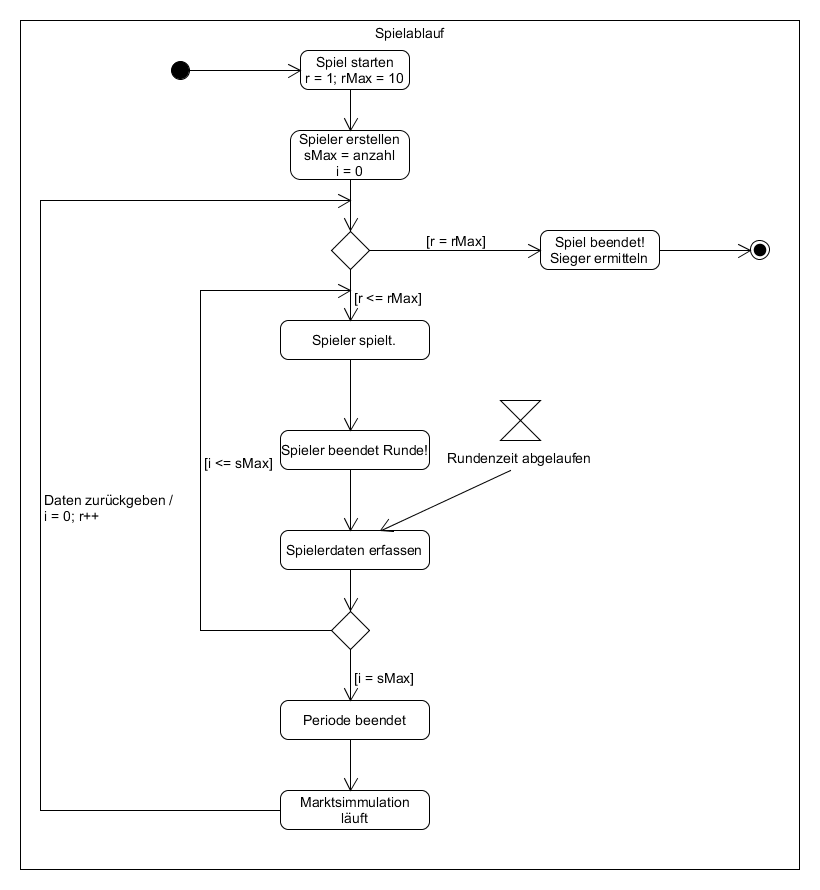
\includegraphics[scale=0.5]{img/Spielablauf.png} 
	\label{key}
	\caption{text}
\end{figure}





